\documentclass[12pt, a4paper]{article}

\usepackage{graphicx}
\usepackage{amsmath, amssymb}
\usepackage[utf8]{inputenc}
\usepackage[T2A]{fontenc}
\usepackage[english, russian]{babel}
\usepackage[margin=2cm]{geometry}
\usepackage[most]{tcolorbox}
\usepackage{caption}
\usepackage{enumitem}

\usepackage{cmap}  
\usepackage{textcomp}          % Дополнительные символы

\tcbuselibrary{breakable}
\tcbset{
  width=0.9\textwidth,
  halign=justify,
  center,
  breakable,
  colback=white
}

\title{Билеты к коллоквиуму по математическому анализу}
\author{VG6}
\date{11 неделя 2025}

\newcommand{\N}{\mathbb{N}}
\newcommand{\Q}{\mathbb{Q}}
\newcommand{\Z}{\mathbb{Z}}
\newcommand{\R}{\mathbb{R}}
\newcommand{\eps}{\varepsilon}

\graphicspath{ {./images/} }

\begin{document}
\maketitle
\tableofcontents
\newpage

\section{Введение}
\subsection{Комплексные числа. Действия над ними. Геометрическое представлние. Алгебраическая и триганометрическая форма записи комплексных чисел. Формула Эйлера, определение $e^z$ через действительную экспоненту и действительные триганометрические функции.}

\subsubsection{Определение и свойства}
\begin{tcolorbox}
\textbf{Определение.} \textit{Комплексными числами} называются числа вида $z = x + iy$, где $x, y \in \R$, а $i$ — \textit{мнимая единица}, обладающая свойством $i^2 = -1$.
\end{tcolorbox}
\begin{itemize}
    \item $x = \operatorname{Re } z$ — \textbf{действительная часть} числа $z$.
    \item $y = \operatorname{Im } z$ — \textbf{мнимая часть} числа $z$.
    \item Если $y = 0$, то $z = x$ — действительное число.
    \item Число $\overline{z} = x - iy$ называется \textbf{комплексно-сопряжённым} к $z$.
\end{itemize}

\begin{tcolorbox}
\textbf{Свойство:} $z \cdot \overline{z} = (x + iy)(x - iy) = x^2 - (iy)^2 = x^2 - i^2y^2 = x^2 + y^2$.
\end{tcolorbox}

\begin{tcolorbox}[title=Важное примечание]
\textbf{Нельзя} сравнивать комплексные числа операциями $<, >, \leq, \geq$!
\end{tcolorbox}

\subsubsection{Арифметические операции}
Пусть $z_1 = x_1 + iy_1$, $z_2 = x_2 + iy_2$.
\begin{enumerate}
    \item \textbf{Сложение/Вычитание:}
    $z_1 \pm z_2 = (x_1 \pm x_2) + i(y_1 \pm y_2)$
    \item \textbf{Умножение:}
    \begin{align*}
    z_1 \cdot z_2 &= (x_1 + iy_1)(x_2 + iy_2) = (x_1x_2 - y_1y_2) + i(x_1y_2 + x_2y_1)
    \end{align*}
    \item \textbf{Деление:}
    \begin{align*}
    \frac{z_1}{z_2} &= \frac{(x_1 + iy_1)(x_2 - iy_2)}{(x_2 + iy_2)(x_2 - iy_2)} = \frac{(x_1x_2 + y_1y_2) + i(x_2y_1 - x_1y_2)}{x_2^2 + y_2^2}\\
    \end{align*}
\end{enumerate}

\subsubsection{Геометрическое представление}
\begin{centering}
    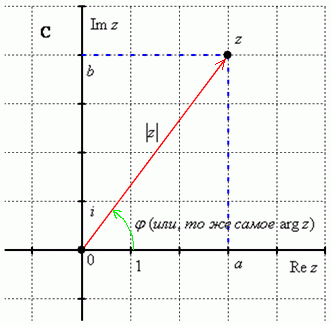
\includegraphics[width=0.4\linewidth]{complex_numbers/compl_plane.png}
\end{figure}

\subsubsection{Тригонометрическая форма}
\begin{tcolorbox}[nobreak]
	\[ z = r(cos\phi +i\; sin\phi),\; r=|z| \]
\end{tcolorbox}

\[ z_1\cdot z_2 = r_1\cdot r_2 \cdot (cos(\phi_1+\phi_2) + i\; sin(\phi_1+\phi_2)) \]
\[\cfrac{z_1}{z_2} = \cfrac{r_1}{r_2}(cos(\phi_1-\phi_2) + i\; sin(\phi_1-\phi_2)) \]

\subsubsection{Формула Эйлера}
\begin{tcolorbox}
	\[ e^{i\phi} = cos\phi +isin\phi \]
	\[ e^z = e^{x+iy} = e^x\cdot e^{iy} = e^x \cdot (cos\; y +i\cdot sin\; y) \]
\end{tcolorbox}

Действительная часть: $ Re\ e^z = e^x \cos y$\\
Мнимая часть: $Im\ e^z = e^x \sin y$


\subsection{Возведение в степень и извлечение корня из комплексных чисел. Форула Муавра.}

\subsubsection{Формула Де-Муавра}
\begin{tcolorbox}
\[ (cos \phi +i\; sin\phi)^k = cos\; k\phi + i\; sin\; k\phi \]
\end{tcolorbox}

\subsubsection{Комплексные корни}
\[ \sqrt[n]{z} = \omega \]
\[ \omega^n = z, z \not= 0\]
\[ z = re^{i\phi}, \omega = \rho e^{i\Psi}  \]
\[ \omega^n = \rho^n e^{in\Psi} = z = re^{i\phi} = re^{i(\phi+2\pi k)}\]
\begin{tcolorbox}
\[ \rho^n = r \Rightarrow \rho = \sqrt[n]{r} \]
\[ n\Psi = \phi + 2\pi k \Rightarrow \Psi = \cfrac{\phi}{n} + \cfrac{2\pi}{n}k \]
\end{tcolorbox}
Корни будут образовывать правильный многоугольник.\\
\begin{centering}
	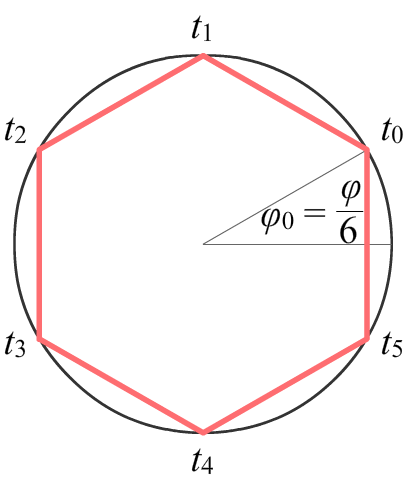
\includegraphics[width=0.2\linewidth]{complex_numbers/roots_of_complex_numbers.png}
\end{centering}

\subsection{Неравенство треугольника для действительных и комплексных чисел, геометрическое и алгебраическое доказательства.}

\subsubsection{Неравенство треугольника}
\begin{figure}[h]
    \centering
    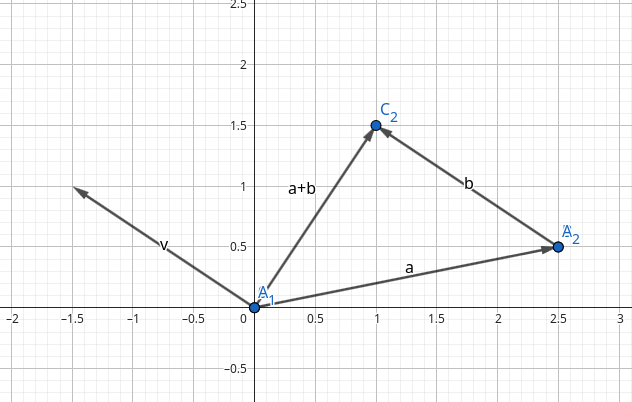
\includegraphics[width=0.5\linewidth]{images/Неравенство(вектора).png}
    \caption{Геометрический смысл неравенства треугольника: длина стороны \( |\vec{a} + \vec{b}| \) не превосходит суммы длин сторон \( |\vec{a}| + |\vec{b}| \).}
    \label{fig:triangle}
\end{figure}
\begin{tcolorbox}
\textbf{Теорема (Неравенство треугольника):}
Для любых комплексных чисел $z_1, z_2$ справедливо:
$$|z_1 + z_2| \leq |z_1| + |z_2|$$
\end{tcolorbox}

\begin{tcolorbox}[title=Доказательство, breakable]
$|a+b| \leq |a| + |b|$
\begin{enumerate}
    \item $a \geq 0\ (|a| \geq |b|)$ \\
    $a + b \geq 0$, то $|a+b| = a+b$.\\
    $a + b \leq 0$, то $|a+b| = -(a+b) = -a-b \leq |a|+|b|$
    \item $|a-b| \geq ||a|-|b||$\\
    $a = (a - b) + b$ по н.т.: $|a + 0| \leq |a-b|+|b| \Rightarrow |a-b| \geq |a|-|b|$ \\
    Аналогично $|b| \leq |b-a|+|a| \Rightarrow |a-b| \geq |b|-|a|$ \\
    Получим, что 
    $
    \begin{cases}
        |a-b| \geq |a|-|b|\\
        |a-b| \geq |-(|a|-|b|)
    \end{cases}
    \Rightarrow |a-b| \geq ||a|-|b||
    $
\end{enumerate}
\end{tcolorbox}

\begin{tcolorbox}[title=Следствие, breakable]
$$||z_1| - |z_2|| \leq |z_1 \pm z_2| \leq |z_1| + |z_2|$$
\end{tcolorbox}

\subsection{Метод математической индукции (ММИ). Прямая индукция. Формула Бинома Ньютона}

\subsubsection{Метод математической индукции (ММИ)}
\begin{tcolorbox}
\textbf{Алгоритм доказательства по индукции:}
\begin{enumerate}
    \item \textbf{База индукции:} Проверить утверждение для $n = 1$.
    \item \textbf{Индукционное предположение:} Предположить, что утверждение верно для $n = k$.
    \item \textbf{Индукционный переход:} Доказать, что из этого следует верность утверждения для $n = k+1$ (Прямая индукция).
\end{enumerate}
\end{tcolorbox}

\subsubsection{Бином Ньютона}
\begin{tcolorbox}
\textbf{Определение.}\\
\textit{Биномиальный коэффициент}:
$C_n^k = \dfrac{n!}{k!(n-k)!}$, где $n,k \in \mathbb{N}_0$\\
\end{tcolorbox}

\begin{tcolorbox}
\textbf{Формула бинома Ньютона:}
$$(a+b)^n = \sum_{k=0}^{n} C_n^k a^{n-k}b^k$$
\end{tcolorbox}

\begin{tcolorbox}[title=Доказательство по ММИ, breakable]
\textbf{База индукции:} Для $n=1$:
$$(a+b)^1 = a + b$$
$$\sum_{k=0}^{1} C_1^k a^{1-k}b^k = C_1^0 a^1 b^0 + C_1^1 a^0 b^1 = 1 \cdot a \cdot 1 + 1 \cdot 1 \cdot b = a + b$$
База индукции доказана.

\textbf{Индукционное предположение:} Предположим, формула верна для $n = m$:
$$(a+b)^m = \sum_{k=0}^{m} C_m^k a^{m-k}b^k$$

\textbf{Индукционный переход:} Докажем для $n = m+1$.
Рассмотрим левую часть:
$$(a+b)^{m+1} = (a+b) \cdot \sum_{k=0}^{m} C_m^k a^{m-k}b^k$$
Раскроем скобки:
$$= \sum_{k=0}^{m} C_m^k a^{m+1-k}b^k + \sum_{k=0}^{m} C_m^k a^{m-k}b^{k+1}$$
Во второй сумме сделаем замену индекса $j = k+1$:
$$= \sum_{k=0}^{m} C_m^k a^{m+1-k}b^k + \sum_{j=1}^{m+1} C_m^{j-1} a^{m+1-j}b^{j}$$
Теперь объединим суммы, выделяя крайние слагаемые:
$$= C_m^0 a^{m+1} + \sum_{k=1}^{m} \left[ C_m^k + C_m^{k-1} \right] a^{(m+1)-k}b^k + C_m^m b^{m+1}$$
Используем свойство биномиальных коэффициентов:
$$C_m^k + C_m^{k-1} = C_{m+1}^k$$
Учитывая, что $C_m^0 = C_{m+1}^0 = 1$ и $C_m^m = C_{m+1}^{m+1} = 1$, получаем:
$$(a+b)^{m+1} = \sum_{k=0}^{m+1} C_{m+1}^k a^{(m+1)-k}b^k$$
Индукционный переход завершён.
\end{tcolorbox}

\subsection{ММИ. Обратная индукция. Неравенство между средним арифметическим и средним геометрическим.}

\subsubsection*{Неравенство о средних}
\begin{tcolorbox}
\textbf{Теорема (Неравенство между средним арифметическим и средним геометрическим):}
Для любых $a_1, a_2, \dots, a_n \geq 0$ справедливо:
$$\frac{a_1 + a_2 + \dots + a_n}{n} \geq \sqrt[n]{a_1 a_2 \dots a_n}$$
Равенство достигается тогда и только тогда, когда $a_1 = a_2 = \dots = a_n$.
\end{tcolorbox}

\begin{tcolorbox}[title=Доказательство по ММИ (метод Коши / метод обратой индукции), breakable]
Докажем теорему в три этапа.

\textbf{1. База индукции для степеней двойки ($n=2^m$).}
\begin{itemize}
    \item \textbf{Для $n=2$:} Докажем $\frac{a_1 + a_2}{2} \geq \sqrt{a_1 a_2}$.
    $$(a_1 - a_2)^2 \geq 0 \Rightarrow a_1^2 - 2a_1a_2 + a_2^2 \geq 0 \Rightarrow a_1^2 + 2a_1a_2 + a_2^2 \geq 4a_1a_2 \Rightarrow$$
    $$\Rightarrow (a_1 + a_2)^2 \geq 4a_1a_2 \Rightarrow \frac{a_1 + a_2}{2} \geq \sqrt{a_1 a_2}$$
    \item \textbf{Предположим, неравенство верно для $n = k$.}
    \item \textbf{Докажем для $n = 2k$:}
    $$\frac{a_1 + \dots + a_{2k}}{2k} = \frac{\frac{a_1 + \dots + a_k}{k} + \frac{a_{k+1} + \dots + a_{2k}}{k}}{2} \geq$$
    $$\geq \frac{\sqrt[k]{a_1 \dots a_k} + \sqrt[k]{a_{k+1} \dots a_{2k}}}{2} \geq \sqrt{\sqrt[k]{a_1 \dots a_k} \cdot \sqrt[k]{a_{k+1} \dots a_{2k}}} = \sqrt[2k]{a_1 \dots a_{2k}}$$
\end{itemize}

\textbf{2. Докажем, что если неравенство верно для $n$, то оно верно и для $n-1$.}
Рассмотрим $a_1, a_2, \dots, a_{n-1} \geq 0$. Пусть
$$a_n = \frac{a_1 + a_2 + \dots + a_{n-1}}{n-1}$$
Для набора из $n$ чисел неравенство верно:
$$\frac{a_1 + \dots + a_{n-1} + a_n}{n} \geq \sqrt[n]{a_1 a_2 \dots a_{n-1} a_n}$$
Подставим $a_n$:
$$\frac{(a_1 + \dots + a_{n-1}) + \frac{a_1 + \dots + a_{n-1}}{n-1}}{n} = \frac{a_1 + \dots + a_{n-1}}{n-1} = a_n$$
Таким образом:
$$a_n \geq \sqrt[n]{a_1 a_2 \dots a_{n-1} a_n}$$
Возведём в степень $n$:
$$a_n^n \geq a_1 a_2 \dots a_{n-1} a_n \Rightarrow a_n^{n-1} \geq a_1 a_2 \dots a_{n-1}$$
Извлекая корень $(n-1)$-й степени:
$$a_n \geq \sqrt[n-1]{a_1 a_2 \dots a_{n-1}} \Rightarrow \frac{a_1 + \dots + a_{n-1}}{n-1} \geq \sqrt[n-1]{a_1 a_2 \dots a_{n-1}}$$

\textbf{3. Завершение доказательства.}
Мы доказали, что:
\begin{enumerate}
    \item Неравенство верно для $n=2$ (а значит, для $n=4,8,16,\dots$)
    \item Из верности для $n$ следует верность для $n-1$
\end{enumerate}
Следовательно, неравенство верно для любого натурального $n$.
\end{tcolorbox}

\section{Действительные чсла. Числовые множества.}
\subsection{Дедекиндовы сечения. Определение действительных чисел по Дедекинду. Полнота $\R$ по Дедекинду. (Полноты я не нашёл)}

\subsubsection{Неполнота рациональных чисел.}
$r = \cfrac{p}{q},p\in \Z,q\in\N $\\
Дробь можно сделать несократимой.\\
Пусть $(\cfrac{p}{q})^2 = 2$ - несократимая дробь $\Rightarrow p^2 = 2q^2 \Rightarrow p = 2k$ (p - чётное число) \\
$k^2 = 2q^2 \Rightarrow q^2 = 2k^2 \Rightarrow $ q - чётное число
\\т.к. дробь несократимая, а числитель и знаменатель чётные, то она на самом деле сократимая. Противоречие! \\
Значит это число \textbf{нельзя} представить рациональной дробью.
\begin{figure}[h]
    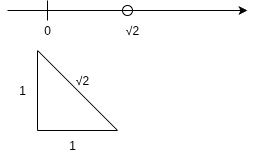
\includegraphics[width=0.2\linewidth]{images/Дедекиндовы сечения/Начало дедекиндовых сечений.png}
\end{figure}\\
Если на оси отметить все рациональные числа точками, то $\sqrt{2}$ - будет выколотой точкой.
\subsubsection*{Отрезки}
$I_n = [a_n, b_n] = \{ r \in \Q\; |\; a_n \leq r \leq b_n \}$, где $a_n, b_n \in \Q$
\begin{tcolorbox}
Будем считать, что $\forall n [a_{n+1}, b_{n+1}] \subset [a_n, b_n]$ - \textbf{вложенные отрезки.}\\
Это значит, что $a_n \leq a_{n+1} \leq b_{n+1} \leq b_n$ и следующий отрезок меньше предыдущего.
\end{tcolorbox}
\begin{tcolorbox}
    $b_n - a_n \xrightarrow{n\to\infty} 0$ - \textbf{стягивающиеся отрезки.}
\end{tcolorbox}
\textbf{Дальше будем подразумеваться}, что все последовательности $\{I_n\}$ - вложенные и стягивающиеся в точку.
\begin{figure}[h]
    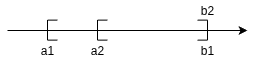
\includegraphics[width=0.25\linewidth]{images/Дедекиндовы сечения/Смысл отрезков.png}
\end{figure}\\
Что нам дают такие отрезки: $\forall r$ \\
\begin{equation}
    \exists n: r < a_n \Rightarrow \forall m > n:\; r < a_m
\end{equation}
\begin{equation}
    \exists n: r > b_n \Rightarrow \forall m > n:\; r > b_m
\end{equation}
\begin{equation}
    \forall n: a_n \leq r \leq b_n
\end{equation}
\begin{enumerate}
    \item левый класс для $\{I_n\}$ (всегда не пуст)
    \item правый класс для $\{I_n\}$ (всегда не пуст)
    \item центральный класс для $\{I_n\}$ (может быть пустым учитывая $r \in \Q)$. Не может содержать более 1 Q числа.
\end{enumerate}
Слово "класс" подразумевает множество.
\begin{tcolorbox}
    \textbf{Дедекиндово сечение}  - множество рациональных чисел (Q) порождённое последовательностью $\{I_n\}$.
\end{tcolorbox}
Тогда каждому действительному числу будет соответствовать своё дедекиндово сечение.

\begin{tcolorbox}
\textbf{Определение}\\
\textit{$\{I_n\}$ и $\{I_n``\}$ - \textbf{эквиваленты}, если они порождают одинаковые разбиения на классы}
\end{tcolorbox}

\begin{tcolorbox}
\textbf{Теорема 1}\\
$\{ I_n \}\sim$ эквивалентна $\{ I_n` \} \Leftrightarrow$
\begin{enumerate}
    \item $\forall n \;\; a_n - a_n` \xrightarrow{n \to \infty} 0 $\\
    ИЛИ
    \item $\forall n a_n \leq b_n`,\; a_n` \leq b_n$
\end{enumerate}
\end{tcolorbox}

\begin{tcolorbox}[title=Доказательство Т1, breakable]
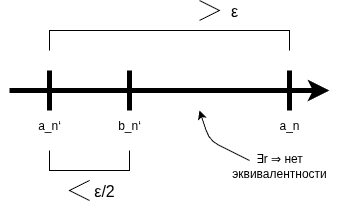
\includegraphics[width=0.4\linewidth]{images/Дедекиндовы сечения/Доказательство Т1.png}\\
\textbf{Только п.1.} \\
$\Rightarrow$: $\{ I_n \} \sim \{ I_n` \} \Rightarrow a_n-a_n` \rightarrow 0$\\
от противного: тогда $a_n-a_n` \nrightarrow 0 \Leftrightarrow \\ 
\exists \eps>0:\; \forall N\;\; \exists n > N\; |a_n - a_n`| \geq \eps $ \\
$\Rightarrow $ для бесконечно многих номеров либо $a_n-a_n` > \eps$, либо $a_n` - a_n > \eps$\\
Пусть для бесконечно многих номеров $a_n - a_n` > \eps$ \\
$\exists n_\eps$ длина $[a_n`, b_n`] < \cfrac{\eps}{2}$\\
$b_n`-a_n` \rightarrow 0 \; \exists n_\eps: \; \forall n > n_\eps\; |b_n`-a_n`| < \cfrac{\eps}{2}$\\
Т.к. $\exists r \in [b_n`, a_n]$, то она принадлежит правому классу $\{I_n`\}$ и левому классу $\{I_n\}$. Последовательности не эквивалентны.\\

$\Leftarrow: a_n - a_n`\; \xrightarrow{n\rightarrow \infty} 0 \Rightarrow \{ I_n \} \sim \{ I_n` \}$\\
От противного: пусть $\{ I_n \} \nsim \{ I_n` \}$, то есть $\exists r \in Q\; r$ из левого класса для одной и центрального или правого класса другой.

r из левого класса $\{ I_n \} \exists n: r < a_n$
\begin{enumerate}
    \item[i.] r из правого класса $\{ I_n` \} \Rightarrow \exists n`: \forall n > n`\;\; a_n` \leq b_n` < r < a_n \leq a_m$\\
    \item[ii.] r из центрального класса $\{ I_n` \}$\\
    $\exists n: r < a_n$ Пусть $\eps = a_n - r(>0)$\\
    $\exists n_\eps: \forall m > n_\eps |b_m`-a_m`| < \cfrac{\eps}{2} \Rightarrow [a_m`,b_m`]$ на расстоянии не меньше $\cfrac{\eps}{2}$ от $a_n$
\end{enumerate}

\textbf{2 вариант доказательства в обратную сторону.}\\
$\Leftarrow: a_n - a_n`\; \xrightarrow{n\rightarrow \infty} 0 \Rightarrow \{ I_n \} \sim \{ I_n` \}$\\
а) совпадение левых классов $r \in $ левый класс для $\{I_n\}$
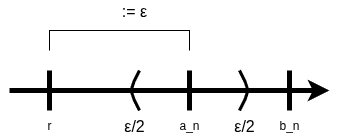
\includegraphics[width=0.4\linewidth]{images/Дедекиндовы сечения/Доказательство Т1.2.png}\\
$\exists n: r < a_n$\\
$\exists n_\eps: \forall n>n_\eps \;\;|a_n-a_n`| < \cfrac{\eps}{2} \Rightarrow r < a_n` \Rightarrow r\ \in $ левый класс для $\{I_n`\}$ \\
б) правые классы аналогично
\end{tcolorbox}

\subsubsection{Ограничение на количество элементов центрального класса.}
Если r из центрального класса, то $\forall n: \; a_n \leq r \leq b_n$\\
А если $\exists r`,r \in $ центральный класс $r<r`$, то $a_n \leq r < r` \leq b_n$. Тогда длина отрезка не может быть меньше длины отрезка $[r,r`]$ значит она не стремится к 0.\\
В центральном классе может быть либо 1 число либо 0.
\subsubsection*{Пример 2-х последовательностей стягивающихся к 0}
$\{I_n\} = [\cfrac{1}{2n},\cfrac{1}{2n}]\;\; \{I_n`\} = [\cfrac{1}{2n+1},\cfrac{1}{2n+1}] \;\; \{I_n``\} = [0,\cfrac{1}{2n+1}]$ Они определяют 1 и то же число.
\subsubsection*{Пример 2-х последовательностей стягивающихся к $\sqrt{2}$}
$[\sqrt{2} - \cfrac{1}{n}, \sqrt{2} + \cfrac{1}{n}]$
\subsubsection{Действительные числа}
\begin{tcolorbox}
\textit{\textbf{Действительные числа} - это вложенные стягивающиеся отрезки с рациональными концами. Числа равны, если последовательность $\{I_n\} \sim \{I_n`\}$  }\\
\textit{\textbf{Действительные число} - отождествляется с дедекиндовым сечением, порождённым $\{[a_n, b_n]\}$ . Числа равны, если последовательность $\{[a_n, b_n]\} \sim \{[a_n`, b_n`]\}$  }
\end{tcolorbox}

\subsubsection*{Ограничение на количество элементов центрального класса.}
Если r из центрального класса, то $\forall n: \; a_n \leq r \leq b_n$\\
А если $\exists r`,r \in $ центральный класс $r<r`$, то $a_n \leq r < r` \leq b_n$. Тогда длина отрезка не может быть меньше длины отрезка $[r,r`]$ значит она не стремится к 0.\\
В центральном классе может быть либо ё число либо 0.
\subsubsection*{Пример 2-х последовательностей стягивающихся к 0}
$\{I_n\} = [\cfrac{1}{2n},\cfrac{1}{2n}]\;\; \{I_n`\} = [\cfrac{1}{2n+1},\cfrac{1}{2n+1}] \;\; \{I_n``\} = [0,\cfrac{1}{2n+1}]$ Они определяют 1 и то же число.
\subsubsection*{Пример 2-х последовательностей стягивающихся к $\sqrt{2}$}
$[\sqrt{2} - \cfrac{1}{n}, \sqrt{2} + \cfrac{1}{n}]$

\subsection{Лемма об отделимости.}

\subsection{Точная верхняя и нижняя грани ограниченных множеств из В. Теорема Вейерштрасса о существовании точной верхней грани ограниченного сверху множества как следствие леммы об отделимости (принцип полноты В по Вейерштрассу).}

\begin{tcolorbox}
    \textbf{Принцип полноты множества по Вейерштрассу}
    Принцип полноты множества по Вейерштрассу означает, что любое ограниченное сверху множество имеет точную верхнюю грань     
\end{tcolorbox}

\begin{tcolorbox}
    \textbf{Определение}
    $\{a_n\}$ монотонна, если возрастает/ строго возрастает/убывает/строго убывает.
\end{tcolorbox}

\begin{tcolorbox}
    \textbf{Теорема по Вейерштрассу}
    \begin{enumerate}
        \item $\{a_n\} \uparrow \; \Rightarrow a_n \to sup\{ a_n \}$
        \item $\{a_n\} \downarrow \; \Rightarrow a_n \to inf\{ a_n \}$
    \end{enumerate}
\end{tcolorbox}

\begin{tcolorbox}
    \textbf{Определение}
    $sup \{a_n\}$ - это $sup$ множества членов последовательности.
\end{tcolorbox}

\begin{tcolorbox}[title=Доказательство полноты $\R$ по Вейерштрассу]
    \textbf{Доказательство}
    \begin{enumerate}
        \item Ограничено сверху $\exists M: \forall n a_n \leq M \Rightarrow \exists sup\{a_n\} = M \in \R$\\
        По определению предела $\forall \varepsilon > 0 \exists n_\varepsilon: \forall n > n_\varepsilon |a_n - M| < \varepsilon $\\
        $\Leftrightarrow M-\varepsilon<a_n<M+\varepsilon$ т.к. $M=sup\{a_n\}$, то $a_n \leq M$ надо проверить $M-\varepsilon<a_n\leq M$\\
        M - наименьшая верхняя грань $\Rightarrow \exists n_\varepsilon: \forall n > n_\varepsilon \;\;\;\;\; M-\varepsilon \leq a_{n_\varepsilon} \leq a_n \leq M $\\
        т.е. по определению 
        \[M = \lim_{n\to\infty} a_n\]
        \textbf{Следствие} $\{a_n\}$ - монотонна $\{a_n\}$ - сходится $\Leftrightarrow \{a_n\}$ - ограничена.
    \end{enumerate}
\end{tcolorbox}

\subsection{Последовательности стягивающихся отрезков с действительными концами. Теорема Кантора о стягивающихся отрезках с действительными концами (принцип полноты ® по Кантору).}

\subsection{Полнота К по Дедекинду как следствие принципа стягивающихся отрезков.}

\subsection{Счётность множества, рациональных чисел и несчётность множества действительных чисел.}



\section{Последовательность и ряды.}

\subsection{Свойства сходящихся последовательностей (сходимость постоянной последовательности, единственность предела, ограниченность сходящейся последовательности).}

\subsubsection{Предел последовательности}
\begin{tcolorbox}
\textbf{Определение.} Число $a$ называется \textit{пределом последовательности} $\{a_n\}$, если
$$\forall \eps > 0\ \exists N_\eps \in \N\ \forall n > N_\eps: |a_n - a| < \eps$$
Обозначение: $\lim_{n\to\infty} a_n = a$ или $a_n \to a$ при $n \to \infty$.
\end{tcolorbox}

\subsection{Сходимость постоянной последовательности}
\begin{tcolorbox}
    \textbf{Теорема 1.} Если $\exists N: \forall n > N \;\; a_n = a \Rightarrow a_n\to a$
\end{tcolorbox}
\begin{tcolorbox}[title=Доказательство]
    \[ \forall \varepsilon>0 \;\;\forall n>N \;\; |a_n - a| = 0 < \varepsilon \Rightarrow a_n\to a\] по определению 
\end{tcolorbox}

\begin{tcolorbox}
    \textbf{Теорема 2.} Если $ a_n\to a,\;\; b_n\to b \;\;\;\forall n > N \;\; a_n \leq b_n \Rightarrow a\leq b $
\end{tcolorbox}
\begin{tcolorbox}[title=Доказательство]
    \textbf{От противного:}\\ 
    Пусть $ a < b$
\end{tcolorbox}
\textbf{НАДО ПОСМОТРЕТЬ ПРЕДЫДУЩИЕ ЛЕКЦИИ. ЭТО ОТТУДА.}

\subsubsection{Теорема о единственности предела.}
\textbf{Теорема:} Последовательность не может иметь более одного предела.

\begin{tcolorbox}[title=Доказательство теоремы, breakable]
\textbf{Доказательство от противного:}
Предположим, что последовательность $\{a_n\}$ имеет два различных предела: $a_n \to A$ и $a_n \to B$, где $A \neq B$.
Пусть $\eps = \frac{|A - B|}{4} > 0$. Тогда по определению предела:
\begin{itemize}
    \item $\exists N_1: \forall n > N_1: |a_n - A| < \eps$
    \item $\exists N_2: \forall n > N_2: |a_n - B| < \eps$
\end{itemize}
Возьмём $n > \max(N_1, N_2)$. Тогда выполняются оба неравенства. Оценим разность $|A - B|$:
$$|A - B| = |(A - a_n) + (a_n - B)| \leq |A - a_n| + |a_n - B| < \eps + \eps = 2\eps = \frac{|A - B|}{2}$$
Получили противоречие: $|A - B| < \frac{|A - B|}{2}$. Следовательно, наше предположение неверно, и предел единственен.
\end{tcolorbox}

\subsubsection{Ограниченные и сходящиеся последовательности}

\begin{tcolorbox}
\textbf{Определение}
$\{a_n\}$  \textit{ограничена}, если $\exists M>0: \forall n\ |a_n|<M,\ a_n, M, n \in Q$
\end{tcolorbox}

\begin{tcolorbox}
\textbf{Определение}
$\{a_n\}$  \textit{не ограничена}, если $\forall M>0: \exists n\ |a_n|\geq M,\ a_n, M, n \in Q$ 
\end{tcolorbox}

\begin{tcolorbox}
\textbf{Теорема 2} \textit{Любая сходящаяся последовательность ограничена} \\
Если $\{a_n\}$ сходиться $\Rightarrow \{a_n\}$ ограничена
\end{tcolorbox}

\begin{tcolorbox}[title=Доказательство Т2, breakable]
\[\eps := 1\ \exists N: \forall n > N\ \ |a_n-a| < 1 \Leftrightarrow -1<a_n-a<1 \Leftrightarrow a-1 < a_n < a+1  \]
\[ M:= max\{ |a_1|, |a_2|, ..., |a_N|, |a-1|, |a+1| \} + 1\]
$\Rightarrow \{a_n\}$ - ограничена (сверху)
\end{tcolorbox}

\begin{tcolorbox}
\textbf{Определение}
$\{a_n\}$  \textit{ограничена сверху, если} $\exists M: \forall n$ $a_n < M$
\end{tcolorbox}

\begin{tcolorbox}
\textbf{Определение}
$\{a_n\}$  \textit{ограничена снизу, если} $\exists m: \forall n$ $a_n < m$
\end{tcolorbox}

Пример:
\begin{enumerate}
    \item $\{\cos n\}\ |\cos n| \leq 1$
    \item $\{n\}$ ограничена снизу но не сверху (0, 1, ...)
\end{enumerate}

\subsection{Предельный переход в неравенствах для последовательностей.}
\subsection{Теорема о зажатой последовательности (о трёх последовательностях).}
\subsection{Теоремы о сохранении знака сходящейся последовательностью и о сходимости модулей.}
\subsection{Бесконечно малые последовательности, их свойства.}

\begin{tcolorbox}
\textbf{Определение}
\textit{Бесконечно малые последовательности}
\begin{center}
    $\{\alpha_n\}\ (\forall n, \alpha_n \in Q)$ бесконечно малая, если $\alpha_n 
    \xrightarrow{n\rightarrow \infty} 0$    
\end{center}
\end{tcolorbox}

\begin{tcolorbox}
\textbf{Теорема 3} 
\begin{center}
    Если $a_n \rightarrow a \Leftrightarrow a_n = a + \alpha_n$, где $ \{\alpha_n\}$ - б.м.
\end{center}
\end{tcolorbox}

\begin{tcolorbox}[title=Доказательство Т3]
$\Rightarrow$:\\
\[ \forall \eps>0\ \exists n_\eps : \forall n > n_\eps\ |a_n - a| < \eps \]
\begin{center}
    Пусть $ |a_n-a| = \alpha_n \Rightarrow a_n = a + \alpha_n $    
\end{center}
\[ \forall \eps > 0\ \exists n_\eps: \forall n > n_\eps\  |a_n -a| = |\alpha_n - 0| < \epsilon \Leftrightarrow \alpha_n \xrightarrow[n\rightarrow \infty]{} 0 \]
$\Leftarrow$:\\
\begin{center}
    $ \{\alpha_n \} $ - б.м., т.е. $ \forall \eps>0\ \exists n_\eps : \forall n > n_\eps\ \eps > |\alpha_n| = |a_n-a| \Leftrightarrow a_n \xrightarrow[n \rightarrow \infty]{} a$    
\end{center}
\end{tcolorbox}

\begin{tcolorbox}
\textbf{Теорема 4}
\begin{enumerate}
    \item $\{\alpha_n\}$ и $\{\beta_n\}$ - б.м. $\Rightarrow \{\alpha_n \pm \beta_n\}$ - б.м.
    \item $\{\alpha_n\}$ - б.м. и $\{\beta_n\}$ - ограничена $\Rightarrow \{\alpha_n \cdot \beta_n\}$ - б.м.
\end{enumerate}
\end{tcolorbox}

\begin{tcolorbox}[title=Доказательство Т4: Предел суммы/разности б.м. последовательностей, breakable]
\small

\textbf{Доказательство:}
\begin{enumerate}

\item[I] Требуется доказать, что \( \forall \varepsilon > 0\ \exists n_\varepsilon \in \mathbb{N} : \forall n > n_\varepsilon\ |\alpha_n \pm \beta_n| < \varepsilon \).

\begin{enumerate}
    \item[1.] Зафиксируем произвольное \( \varepsilon > 0 \).
    \item[2.] Так как \( \{\alpha_n\} \) — б.м., то для числа \( \frac{\varepsilon}{2} > 0 \) найдётся номер \( n_{\varepsilon}' \) такой, что: $\forall n > n_{\varepsilon}'\quad |\alpha_n| < \frac{\varepsilon}{2}$
    
    \item[3.] Аналогично $\forall n > n_{\varepsilon}''\quad |\beta_n| < \frac{\varepsilon}{2}$
    
    \item[4.] Выберем номер \( n_\varepsilon = \max\{n_{\varepsilon}', n_{\varepsilon}''\} \). Тогда для всех \( n > n_\varepsilon \) будут выполняться \textbf{оба} неравенства из пунктов (2) и (3).
    \item[5.] Оценим модуль суммы (или разности) для всех \( n > n_\varepsilon \), используя неравенство треугольника:
    \[
    |\alpha_n \pm \beta_n| \leq |\alpha_n| + |\beta_n| < \frac{\varepsilon}{2} + \frac{\varepsilon}{2} = \varepsilon
    \]
\end{enumerate}

Так как \( \forall \varepsilon > 0\ \exists n_\varepsilon: \forall n > n_\eps\ |\alpha_n \pm \beta_n| < \varepsilon \), то по определению последовательность \( \{\alpha_n \pm \beta_n\} \) является бесконечно малой.

\item[II] {$\beta_n$} - ограничена $\Rightarrow \exists M > 0:\ \forall n \ |b_n| < M \ \forall\eps > 0\ \exists n_\eps : \forall n > n_\eps\ |\alpha_n| < \cfrac{\eps}{2}$\\
$|\alpha_n \cdot \beta_n|= |\alpha_n| \cdot |\beta_n| \leq \cfrac{\eps}{M} \cdot M = \eps$
\end{enumerate}
\end{tcolorbox}

\begin{tcolorbox}
\textbf{Теорема 5}
\[ a_n \xrightarrow[n\rightarrow \infty]{}a,\ b_n \xrightarrow[n\rightarrow \infty]{}b\]
\begin{enumerate}
    \item $a_n + b_n \xrightarrow[n\rightarrow \infty]{} a + b$
    \item $a_n \cdot b_n \xrightarrow[n\rightarrow \infty]{} a \cdot b$
    \item Если $b_n \ne 0\ \forall n \ nb \ne 0$, то $\cfrac{a_n}{b_n} \xrightarrow[n\rightarrow \infty]{} \cfrac{a}{b}$
\end{enumerate}
\end{tcolorbox}

\begin{tcolorbox}[title=Доказательство Т5: Арифметические свойства предела, breakable]
\textbf{Из Т4 про арифметические свойства б.м. последовательностей}
\begin{enumerate}
    \item $a_n + b_n = (a + \alpha_n) + (b+\beta_n) = (a+b)+(\alpha_n+\beta_n)$\\
    $(\alpha_n+\beta_n)$ - Сумма б.м., $(a+b)+(\alpha_n+\beta_n) = $ по Т3 $= a_n+b_n \rightarrow a + b$
    \item $a_nb_n = (a + \alpha_n) + (b + \beta_n) = ab + (\alpha_nb + \beta_na + \alpha_n\beta_n) \xrightarrow[]{T3} ab$
    \item Докажем, что $\cfrac{a_n}{b_n} - \cfrac{a}{b}$ - б.м.\\
    $\cfrac{a_n}{b_n} - \cfrac{a}{b} = \cfrac{a_nb-ab_n}{b_nb} = \cfrac{(a+\alpha_n)b-a(b+\beta_n)}{bb_n} = \cfrac{\alpha_nb-a\beta_n}{bb_n}$\\
    $\alpha_nb-a\beta_n$ - бесконечно малая\\
    Проверим ограниченность $\cfrac{1}{bb_n}$\\
    $\eps=\cfrac{|b|}{2}: \exists n_\eps\ \forall n>n_\eps\ |b_n-b|<\cfrac{\eps}{2}$\\
    $|b_n| = |b-(b-b_n)| \geq{}$(неравенство треугольника)$\geq ||b|-|b-b_n||\geq|b|-|b-b_n|>\cfrac{|b|}{2}\Rightarrow\cfrac{1}{|b_n|}<\cfrac{2}{|b|} \Rightarrow \{\cfrac{1}{b_n}\}$ - ограничена\\
    Значит, что $\cfrac{a_n}{b_n} - \cfrac{a}{b} = \cfrac{\alpha_nb-a\beta_n}{bb_n}$ - бесконечно малая.
\end{enumerate}
\end{tcolorbox}

\subsection{Бесконечно большие последовательности. Связь бесконечно малых и бесконечно больших последовательностей.}
\subsection{Арифметические свойства сходящихся последовательностей.}
\subsection{Монотонные последовательности. Критерий сходимо}сти монотонной последовательности.
\subsection{Число е как предел последовательности.}

Вспомним неравенство среднего геометрического и среднего арифметического.
\[\forall k: a_k>0\;\;\;\ \sqrt[n]{a_1\cdot a_2\cdot ... \cdot a_n} \leq \cfrac{a_1+a_2+...+a_3}{n} \]
Пусть $a_1 = a > 0,\;a_2=a_3=...=a_{n+1}=d>0$\\
$\sqrt[n+1]{a\cdot b^n} \leq \cfrac{a+nb}{n+1}$\\
$(1+\cfrac{1}{n})^k$ - сходится
\begin{tcolorbox}[title=Доказательства монотонности]
    \begin{enumerate}
        \item $(1+\cfrac{1}{n})^k \uparrow$\\
        Пусть $a = 1,\;b=1+\cfrac{1}{n}$\\
        $\sqrt[n+1]{a\cdot(1+\cfrac{1}{n})^n}\; < \cfrac{1+n(1+\cfrac{1}{n})}{n+1} = \cfrac{n+1}{n+1} = 1+\cfrac{1}{n+1} \uparrow n+1 $
        \begin{tcolorbox}
            \[ (1+\cfrac{1}{n})^n < (1+\cfrac{1}{n+1})^{n+1} \]
        \end{tcolorbox}
        \item $(1-\cfrac{1}{n})^k \uparrow$\\
        Пусть $a = 1,\;b=1-\cfrac{1}{n}$\\
        $\sqrt[n+1]{a\cdot(1-\cfrac{1}{n})^n}\; < \cfrac{1+n(1-\cfrac{1}{n})}{n+1} = \cfrac{n+1-1}{n+1} = 1-\cfrac{1}{n+1} \uparrow n+1 $
        \begin{tcolorbox}
            \[ (1-\cfrac{1}{n})^n < (1-\cfrac{1}{n+1})^{n+1} \]    
        \end{tcolorbox}
        \item $(1+\cfrac{1}{n})^{n+1} = (\cfrac{1}{\frac{n}{n+1}})^{n+1} = \cfrac{1}{(1-\frac{1}{n+1})^{n+1} \downarrow } $
    \end{enumerate}
\end{tcolorbox}
$\forall k,m \;\;\; n=max\{k,m\}$\\
\[ (1+\cfrac{1}{k})^k \leq (1+\cfrac{1}{n})^n < (1+\cfrac{1}{n})^{n+1} \leq (1+\cfrac{1}{m})^{m+1} \Rightarrow \]
$(1+\cfrac{1}{n})^n$ - ограничена сверху $\Rightarrow$ сходится.

\begin{tcolorbox}
    \textbf{Определение} 
    \[e = \lim_{n\to \infty} (1+\cfrac{1}{n})^n \]
\end{tcolorbox}

\begin{tcolorbox}[title=Доказать/подумать]
    \begin{enumerate}
        \item \[ e = \lim_{n\to\infty} (1+\cfrac{1}{1!} +\cfrac{1}{2!} + ... + +\cfrac{1}{n!}) \]
        \item $(1+\cfrac{1}{n})^{n+2}$
        \item Сколько слагаемых нужно взять, чтобы получить e с точностью $10^{-3}$\\
        \item Какое нужно взять n, чтобы получить e с точностью $10^{-3}$
    \end{enumerate}
\end{tcolorbox}

\subsection{Теорема Больцано-Вейерштрасса.}

$n_k$ - строго возрастает последовательность натуральных чисел $\Rightarrow n_k\geq k$ .

\begin{tcolorbox}
    \textbf{Определение} $\forall \{a_n\} \; \{a_n\}$ - подпоследовательность $\{a_n\}$
\end{tcolorbox}
$\{a_n\} = 2^n$, тогда 2, 16, 64, 128 - подпоследовательность\\
$\begin{cases}
    2, \textbf{3}, 4, 16, ...\\
    16, \textbf{2}, 32, ...     
\end{cases}$ - не подпоследовательности\\

\textbf{Теорема Больцано-Вейерштрасса}
\begin{tcolorbox}[]
    $ \forall $ ограниченой $\{a_n\} \exists $сходящаяся подпоследовательность $ \{a_n\} $
\end{tcolorbox}

\begin{figure}[h]
    \centering
    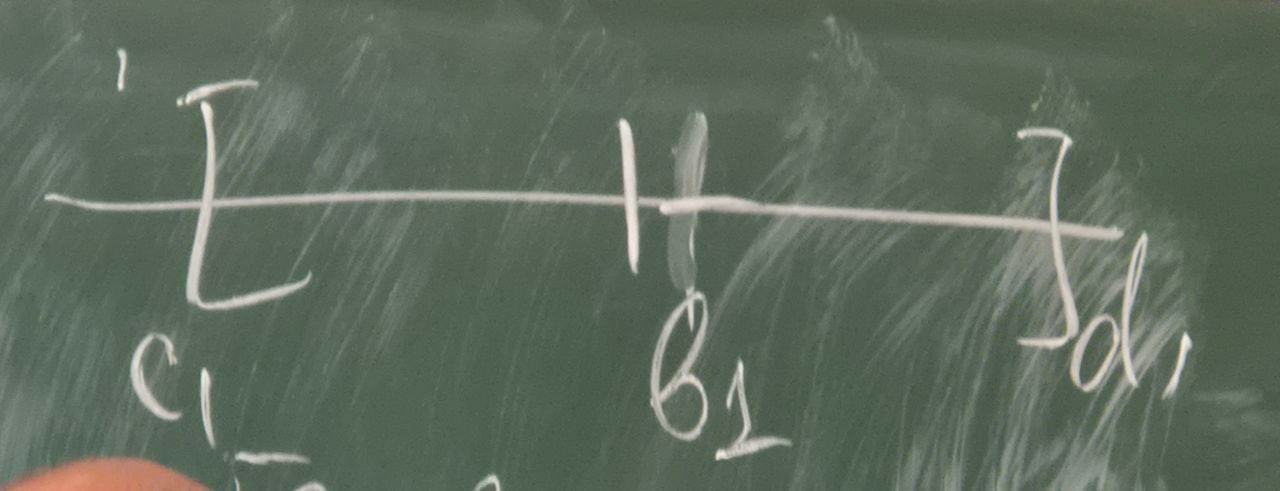
\includegraphics[width=0.5\linewidth]{Т Б-В.png}
\end{figure}

\begin{tcolorbox}[title=Доказательство]
    Прицип вложенных отрезков.\\
    $\exists [c,d]: \forall n\; a_n\in[c,d]$
    \begin{enumerate}
        \item $[c_1,d_2] = [c,d] \;\; \forall a_{n_1} \in [c_2,d_1]$
        \item $b_1 = \cfrac{c_1+d_1}{2}$
                $[c_2,d_2]$ тот из $[c_1,b_1]$ и $[b_1,d_1]$ на котором содержится бесконечно много членов последовательности $\{a_n\}$\\
        $a_{n_2}: a_{n_2} \in [c_2,d_2], n_2>n_1$
        \item $b_2 = \cfrac{c_2+d_2}{2}$\\
        $[c_3,d_3]$ тот из $[c_2,b_2]$ и $[b_2,d_2] ...$\\
        $a_{n_3}: a_{n_3} \in [c_3,d_3], n_3>n_3$

        $\{a_n\} \;\;a_{n_k} \in [c_k,d_k], n_k > n_{k-1}$
        $[c_1,d_1] \supset [c_2,d_2] \supset ... \supset [c_k,d_k] \supset ...$\\
        длина $[c_k,d_k] = \cfrac{1}{2^{k-1}}$
        длина $[c_1,d_1] \to 0$
        $\Leftrightarrow \exists a` = U[c_k,d_k]$\\
        $\forall k\;\; |a_n-a`| \leq \cfrac{1}{2^{k-1}}$ - длина $[c_1,d_1] \to 0$
        $a_{n_k}, a`\in [c_k,d_k] \Rightarrow a_{n_k} \to 0`$
    \end{enumerate}
\end{tcolorbox}

\begin{tcolorbox}
    \textbf{Определение} Частичный предел $\{a_n\}$ - предел $\forall$ сходящейся подпоследовательности $\{a_n\}$
\end{tcolorbox}
\begin{tcolorbox}[title=Следствие из теоремы]
    $\forall \{a_n\} \exists$ подпоследовательность $\{a_{n_k}\}$ которая имеет либо конечное либо бесконечное число пределов.
\end{tcolorbox}
\begin{tcolorbox}[title=Доказательство]
    Если в $\{a_n\} \exists \{a_{n_k}\} a_{n_k} \to a` \in \R$\\
    Если такого нет, то по Теореме Б-В $\{a_{n}\}$ - не ограничена сверху или снизу.\\

    Если $\{a_{n}\} $ - не ограничена сверху:
    \begin{enumerate}
        \item 1 - не верхняя грань $\{a_{n}\}: a_{n_1}: a_{n_1} > 1$
        \item 2 - не верхняя грань $\Rightarrow \exists n_2: a_{n_2}>2, n_2>n_1$
        \item[...]
        \item [k.] $\exists n_k: a_{n_k}>max\{k, a_1, a_2, ..., a_{n_{k-1}}\}, n_k>n_{k-1}$
    \end{enumerate}
\end{tcolorbox}

\subsection{Частичные пределы. Критерий частичного предела.}
\subsection{Критерий Коши существования предела последовательности.}
\begin{tcolorbox}
    $\{a_n\}$ - сходится $\Leftrightarrow \{a_n\}$ - фундаментальна.
\end{tcolorbox}

\begin{tcolorbox}[title=Доказательство]
    Взять с записи
\end{tcolorbox}

\subsubsection{Фундоментальные последовательности.}
\begin{tcolorbox}
    \textbf{Последовательность $\{a_n\} $фундаментальна} - если
    \[\forall \eps>0 \;\; \exists n_\eps : \forall n, m > n_\eps \;\; |a_n-a_m| < \eps\]
    \[ \forall \eps>0 \;\; \exists n_\eps : \forall n > n_\eps,\forall  p \;\; |a_{n+p}-a_n| < \eps \]
\end{tcolorbox}

\subsection{Существование верхнего и нижнего пределов у любой последовательности.}

\textbf{Утверждение 1.} $\forall$ последовательность имеет хотя-бы 1 частичный предел (конечный или бесконечный).
\begin{tcolorbox}[title=Доказательство]
    \begin{enumerate}
        \item Пусть $\{a_n\}$ - не ограничена сверху.\\
        Напоминание: $\{ a_n \}$ - не ограничена сверху, если $\forall M\; \exists a_n > M \Leftrightarrow \exists$ бесконечно много таких членов.\\
        $a_n > 1, a_{n_2} > 2,\ n_2>n_1$\\
        $a_{n_k} > k, n_k > n_{k-1}$\\
        $\{a_{n_k}\} \to +\infty$
        \item Если $\{a_n\}$ не ограничена снизу, то $\exists a_{n_k}\to -\infty$ (аналогично)
        \item Если $\{a_n\}$ - огрничена, то Б-В.
        
    \end{enumerate}
\end{tcolorbox}

\textbf{Утверждение 2.} критерий частичного предела.\\
a - частичный предел $\{a_n\} \Leftrightarrow \forall U_a$ принадлежит б.м. членов последовательности.
\[ \forall U_a \exists a_{n_k}\in U_a^\circ = U_a /\{a\} \] - ЭТО ХУЙНЯ. НАДО НАЙТИ ОШИБКУ\\
На экзамене: что-то может быть.\\

\begin{tcolorbox}[]
    $\forall U_a \; \exists k_{U_a}: \forall k > k_{U_a} \;\; a_{n_k} \in U_a$\\
    $\Rightarrow$ в $U_a$ бесконечно много членов последовательности.\\
    $\Leftarrow$ в $\forall U_a$ бесконечно много членов $\{a_n\}$.\\
    $\eps_1 = \cfrac{1}{2} \;\; U_a = (a-\eps; a+\eps)$ - отсюда любой член $\{a_n\}$\\
    $\eps_2 = \cfrac{1}{2^2} \;\; \exists a_{n_2} \in (a-\eps_2; a+\eps_2), n_2>n_1$\\
    ...\\
    $\eps_k = \cfrac{1}{2^k} \;\; \exists a_{n_k} \in (a-\eps_k; a+\eps_k), n_k>n_{k-1}$\\
    $\{a_{n_k}\} a_{n_k} \to a,$ при $k\to \infty$\\
    $\forall k\;\;\; a-\cfrac{1}{2^n} \to a= a - \eps_k < a_{n_k} < a_\eps = a+ \cfrac{1}{2^k} \to a$\\
    По теореме о зажатой последовательности $a_{n_k} \to \infty$
\end{tcolorbox}

\begin{tcolorbox}
    \textbf{Определене.} \\
    Наибольший из часичных пределов. $\{a_n\}$ - верхний прдел $a_n$\\
    Наименьший из часичных пределов. $\{a_n\}$ - нижний прдел $a_n$
\end{tcolorbox}

\textbf{Теорема} $\forall \{a_n\} \;\; \exists$ верхний и нижний предел.
\begin{tcolorbox}
    \begin{enumerate}
        \item $\exists$ $\underline{\lim} a_n$ - нижний предел $a_n$\\
        Пусть $\{a_n\}$ - не ограничена те $\forall M \exists a_n < M$. Таких $a_n$ - бесконечно много.\\
        $a_{n_1} < -1, a_{n_2} < min\{ -2, a_1, ..., a_{n_1} \} - 1$
        $n_2 > n_1$\\
        $a_{n_k} < min\{-k, a_1, ..., a_{n_{k-1}}\} - 1$\\
        $a_{n_k} - k, n_k > n_{k-1}$\\
        $\{a_{n_k}\}$ - подпоследовательность.\\
        \[ a_{n_k} < -k \Rightarrow a_{n_k} \to -\infty \]
        \item Пусть $\{ a_n \}$ - ограничена снизу.
            \item[a)] $\{a_n\}$  имеет конечные частичные пределы.\\
            A - множество конечных частных пределов. $A \not= \varnothing$ и ограничена снизу.\\
            $\exists inf\; A = a$. Покажем, что $a = \underline{\lim}_{n\to\infty} a_n$
            \begin{center}
                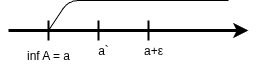
\includegraphics[width=0.2\linewidth]{imageas/Пределы.png}
            \end{center}
            $ \forall \eps > 0 \exists a` \in A $\\
            $a \leq a` < a+\eps$
            \item[б)] $\{a_n\}$ нет конечных частичных пределов.\\
            $a_n \to +\infty$\\
            Если $a_n \not\to +\infty \;\; \exists M: \forall N \;\; \exists n > N\;\;\; a _n\leq M$ \\
            $\exists$ бесконечно много $\{a_n\} < M$ по Б-В $\exists$ конечный частичный предел.
    !!! Каждое действитеьное число является её частиыным пределом.
    \end{enumerate}
\end{tcolorbox}

\subsection{Числовые ряды. Абсолютная и условная сходимость числовых рялов. Критерий Коши сходимости ряда. Необходимое условие сходимости ряда. Признак сравнения.}

\subsubsection{Определения и элементарные факты.}
$ \{a_k\} $ - ЧП
\[ \{a_k\} \to S_n = \sum^n_{k=1}a_k \]
\textbf{Определения}
\begin{tcolorbox}
    \textbf{Определяем бесконечную сумму}.\\
    $\sum^\infty_{k=1} a_k$ - \textbf{ряд}\\
    $a_k$ - \textbf{элемент ряда (общий член)}.\\
    $S_n$ - \textbf{n-ая частичная сумма ряда}.\\
    Если $S_n$ - сходится, то ряд ($\sum^\infty_{1} a_k$) называется \textbf{сходящимся}, $S:=\lim_{n\to\infty} s_n$ - \textbf{суммой ряда}: $\sum_1^\infty = S$.\\
    Если $\{S_n\}$ расходится, то $\sum^\infty_{1} a_k$ - \textbf{расходится}.
\end{tcolorbox}
\subsubsection{\textbf{Теорема 1.}}
\[ \sum_1^\infty a_k \pm \sum_1^\infty b_k = \sum_1^\infty (a_k \pm b_k) \]
\subsubsection{\textbf{Теорема 2. Критерий Коши о сходимости ряда.}}
$ \sum_1^\infty a_k$ - сходится $\Leftrightarrow \forall \eps > 0\;\; \exists n_\eps : \forall n > n\eps \forall p \;\;\; |S_{n+p} - S_n| < \eps $
\[ |\sum_1^{n+p} a_k - \sum_1^n a_k| = |\sum_{n+1}^{n+p} a_k| < \eps \]
\subsubsection{\textbf{Следствие 1. Изменение конечного числа членов ряда не влияет на сходимость.}}
Сумма конечно может измениться, но на сходимость это не влияет.
\subsubsection{\textbf{Следствие 2. Необходимое условие сходимости ряда.}}
Можно считать определением: Если $\sum_1^\infty a_k$ сходится $\Rightarrow a_k \xrightarrow[k\to\infty]{} 0$\\
\begin{tcolorbox}[title=Доказательство]
    $\sum_1^\infty a_k$ - сходится $\forall \eps > 0\; \exists n_\eps:\; \forall n > n_\eps\;\; \forall p \ |\sum_{n+1}^{n+p} a_k| < \eps \Leftrightarrow |a_{n+1}| < \eps$\\
    При p = 1, то есть $\{a_n\}$ - б.м. по определению.
\end{tcolorbox}
\subsubsection*{Пример 1.}
Если |q| < 1
\[ \sum_1^\infty q^k, S_n = 1+...+q^n = \cfrac{1-q^{n+1}}{1-q} \xrightarrow[n\to\infty]{} \cfrac{q}{1-q} \]
\subsubsection*{Пример 2.}
$\sum_1^\infty \cfrac{1}{n}$\\
a, b, c положительные. c - среднее гармоническое a и b, если $\cfrac{2}{c} = \cfrac{1}{a} + \cfrac{1}{b}$\\
$a = \cfrac{1}{n-1}, b = \cfrac{1}{n+1}$\\
$\cfrac{2}{c} = (n - 1) + (n + 1) = 2n$\\
Каждый элемент является средним гармоническим 2-х соседий. По критерию Коши ряд - расходящийся.
\[ |\sum_{n+1}^{n+p} \cfrac{1}{k}| = \cfrac{2}{n+1} + ... + \cfrac{1}{n+p} \geq \cfrac{p}{n+p}\]
Пусть p = n. $\cfrac{p}{n+p} = \cfrac{1}{2}$.
\subsubsection*{\textbf{Пример 3.}}
\[ 1 - 1 + \cfrac{1}{2} - \cfrac{1}{2} + \cfrac{1}{3} - \cfrac{1}{3} + ...\]
$S_{2n} = 0$\\
$S_{2n+1} = \cfrac{1}{n+1} \to 0$\\
А теперь давайте мухлевать. Переставим сумму ряда. Шоу ИМПРОВИЗАЦИЯ!!!\\
$(1+\cfrac{1}{2}) - 1 + (\cfrac{1}{3} + \cfrac{1}{4} +\cfrac{1}{5} + \cfrac{1}{6} + \cfrac{1}{7} + \cfrac{1}{8} + ... + \cfrac{1}{11}) - \cfrac{1}{2}$\\
Берём много положительных слагаемых и вычитаем меньшее по модулю число. Из-за этого ряд расходится.
\subsubsection*{\textbf{Пример 4.}}
\[ \sum^\infty_{0} (-1)^k = (1-1) + (1-1) + ... \]
\[ \sum^\infty_{0} (-1)^k = 1 - (1-1) - (1-1) - ... \]

\subsection{Абсолютно сходящийся ряд.}
\begin{tcolorbox}
    \textbf{Определение.} Если $\sum^\infty_{1} |a_k|$ сходится, то $\sum^\infty_{1} a_k$ сходится абсолютно.
\end{tcolorbox}
\subsubsection{\textbf{Теорема 1. Если ряд сходится абсолютно, то ряд сходится.}}
\begin{tcolorbox}[title=Доказательство (Критерий Коши)]
    По критерию Коши, т.к. $\sum^\infty_{1} |a_k|$ сходится, то $\forall \eps > 0\; \exists n_\eps:\; \forall n > n_\eps\; \forall p\;\; |\sum^{n+p}_{n+1} a_k| \leq |\sum^{n+p}_{n+1} |a_k|| < \eps \Rightarrow$ по критерию Коши $\sum a_k$ сходится.
\end{tcolorbox}
\subsubsection*{\textbf{Пример 1.}}
$1 - 1 + \cfrac{1}{2} - \cfrac{1}{2} + ... $ - сходится, но не абсолютно.
\subsubsection{\textbf{Определение.}} 
Если $\sum^{\infty}_{1} a_k$ сходится, а $\sum^{\infty}_{1} |a_k|$ расходится, то $\sum a_k$ сходится условно.
\subsubsection{\textbf{Теорема 2.}}
$\sum^{\infty}_{1} a_k, \forall k\; a_k \geq 0$\\
$\sum^{\infty}_{1} a_k$ сходится $\Leftrightarrow \{S_N\}$ ограничена.
\begin{tcolorbox}[title=Доказательство]
    \[\forall n\; S_{n+1} = \sum^{n+1}_{1} a_k \geq \sum^{n}_{1} a_k = S_n \]
    $S_n \uparrow$ возрастающая $\{S_n\}$ сходится $\Leftrightarrow$ ограничена.
\end{tcolorbox}
\subsubsection{Теорема 3. Признак сравнения.}
Для комплов не годится.\\
$\sum^{\infty}_{1} a_k,\;\; \sum^{\infty}_{1} b_k,\;\; \forall k\;\; a_k \geq \underline{b_k \geq 0}$\\
Тогда:
\begin{enumerate}
    \item Если $\sum^{\infty}_{1} a_k$ сходится $\Rightarrow \sum^{\infty}_{1} b_k$ сходится.
    \item Если $\sum^{\infty}_{1} a_k$ расходится $\Rightarrow \sum^{\infty}_{1} b_k$ расходится.
\end{enumerate}
\begin{tcolorbox}[title=Доказательство]
Следствие критерия сходимости ряда с неотрицательными членами.\\
\begin{enumerate}
    \item $A_n = \sum^{n}_{1} a_k,\;\; B_n = \sum^{n}_{1} b_k $\\
    $A_n \uparrow,\; B_n \uparrow$ и $A_n \geq B_n$ ($A_n$ можарирует $B_n$)\\
    Если $\sum a_k$ сходится $\Rightarrow \{A_n\}$ ограничена сверху $\Rightarrow \{B_n\}$ ограничена сверху $\Rightarrow \sum b_k$ сходится.
\end{enumerate}
\end{tcolorbox}

\subsubsection{Следствие. (Признак сравнения).}
$\sum a_k,\; \sum b_k \;\; \forall k\; a_k \geq |b_k| > 0$. Не отрицательность $a_k$.\\
Сходимость $\sum a_k \Rightarrow$ сходимость $\sum b_k$ (абсолютная).
\subsubsection*{Пример 1.}
\[\sum^{\infty}_{1} \cfrac{\sin n}{n^2}\]
\[|\cfrac{\sin n}{n^2}| \leq \cfrac{1}{n^2} < \cfrac{1}{(n-1)n}, n \not= 1\]
\[ \cfrac{1}{(n-1)n} = \cfrac{1}{n-1} - \cfrac{1}{n} \]
\[ \sum^{\infty}_{2} \cfrac{1}{n-1)n} = \sum^{\infty}_{2}( \cfrac{1}{-1} - \cfrac{1}{n}) \]
\[ S_n = \sum^{n}_{2} (\cfrac{1}{k-1} - \cfrac{1}{k}) = (\cfrac{1}{2-1} - \cfrac{1}{2}) + (\cfrac{1}{2} - \cfrac{1}{3}) + ... \]

\subsection{Признаки абсолютной сходимости рядов Даламбера и Коши.}

\subsubsection{Теорема 4. Признак Коши.}
\[ \sum_1  a_k\]
\[q = \overline{lim} \sqrt[k]{|a_k|} \]
Тогда:
\begin{enumerate}
    \item $q < 1 \Rightarrow$ абсолютно сходится.
    \item q > 1 расходится
    \item q = 1 ?
\end{enumerate}
\begin{tcolorbox}[title=Доказательство]
    Сравнение с геометрической прогрессией.\\
    \begin{enumerate}
        \item $ 0 \leq q < p < 1 $
        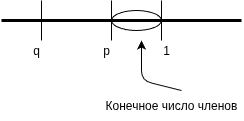
\includegraphics[width=0.5\linewidth]{Ряды/Признак Коши Док-во.png}\\
        $\exists n_p: \forall n>n_p$\\
        $\sqrt[k]{a_k} < p \uparrow \Leftrightarrow |a_k| < p_k$\\
        $\sum^{\infty}_{n+1} p^k$ геометрическая прогрессия с положительным знаком |x|.\\
        $\Rightarrow \sum^{\infty}_{1} a_k$ сходится абсолютно (по признаку сравнения)
        \item q = $\overline{lim} \sqrt[k]{a_k} > 1$\\
        $1 > p > 1$\\
        $\forall$ окрестности $q$ бесконечно много членов $\sqrt[k]{|a_k|} $
    \end{enumerate}
\end{tcolorbox}
\textbf{Замечание.} Признак Коши бесполезно использовать, если ряд не похож на геометрическую прогрессию.\\
\textbf{Запомните.} Признак коши достаточное условие абсолютной сходимости.\\
\textbf{Следствие} Если $ \sqrt[n]{|a_n|} \leq q < 1 \Rightarrow \exists q,N\; \forall n > N: \;  \sum a_n$ сходится абсолютно

\textbf{Пример.} $ \sum^\infty_{n=1} (2+(-1)^n)^n \cdot z^n$\\
\[
	\sqrt[n]{((2+(-1)^n)^n z^n} = (2+(-1)^n)|z|\\
	n = 2k: \sqrt[n]{|a_n|} = 3|z| = \overline{\lim} \sqrt[n]{|a_n|} \\
	n = 2k+1: \sqrt[n]{|a_n|} = |z|\\ 
\]
Если: 
	$3|z| < 1$ сходится $|z| < \cfrac{1}{3}$\\
	$3|z| > 1$ расходится $|z| > \cfrac{1}{3}$\\
	$3|z| = 1 |z| = \cfrac{1}{3} $

\textbf{Теорема 5. Признак д-Аламбера}\\
!Он всегда слабее признака Коши.
\begin{tcolorbox}
	\[
		\sum_{n=1}^{\infty}: |\cfrac{a_{n+1}}{a_{n}}| \to q
	\]
\begin{enumerate}
	\item $q < 1 \Rightarrow$ абсолютно сходится
	\item $q < 1 \Rightarrow$ расходится
	\item $q = 1 \Rightarrow$ Ничего не даёт
\end{enumerate}
\end{tcolorbox}

\begin{tcolorbox}[title=Доказательство.]
	\begin{enumerate}
		\item  Сравнение с геометрической прогрессией.\\
		$\exists n_p: \forall n > n_p \;\; |\cfrac{a_{n + 1}}{a_n}| < p$\\
		Пусть для $\forall n$\\
		$ a_{n+1} = \cfrac{a_{n+1}}{a_n} \cdot  \cfrac{a_{n}}{a_{n-1}} \cdot ... \cdot \cfrac{a_{2}}{a_1} $
		$ |a_{n+1}| = |\cfrac{a_{n+1}}{a_n}| \cdot  |\cfrac{a_{n}}{a_{n-1}}| \cdot ... \cdot |\cfrac{a_{2}}{a_1}| \cdot |a_1| < p^n |a_1| $\\
		$ \displaystyle\sum_{}^{} p^n |a_1|$ сходится (геометрическая прогрессия)
	\item $\exists N: |\cfrac{a{_n+1}}{a_n}| > 1\;\; \forall n > N$\\
		Пусть $ \forall N\; |\cfrac{a_{n+1}}{a_n}| > 1 $\\
		$ |a_{n+1}| > |a_{n}| > |a_{n-1}| > ... |a_{1}| > 0 \Rightarrow a_n \not\to 0$
	\item $ \displaystyle\sum_{1}^{\infty} \cfrac{1}{n}\;\; |\cfrac{a_{n+1}}{n}| = \cfrac{n}{n+1} \to 1$\\
		$ \displaystyle\sum_{1}^{\infty} \cfrac{1}{n^2}\;\; |\cfrac{a_{n+1}}{n}| = \cfrac{n^2}{(n+1)^2} \to 1$\\
 	\end{enumerate}
\end{tcolorbox}

\textbf{Следствие.} $\forall n > N:\; |\cfrac{a_{n+1}}{a_n}| \leq q < 1 \Rightarrow \sum a_n$ сходится абсолютно.

\begin{tcolorbox}[title=Доказательство следствия]
	Пусть $ \forall n\; |\cfrac{a_{n+1}}{a_n}| \leq q < 1 $\\
$ |a_{n+1}| = |\cfrac{a_{n+1}}{a_n} \cdot |\cfrac{a_{n}}{a_{n-1}} \cdot ... \cdot |\cfrac{a_{2}}{a_1} \cdot |a_1| \leq q^n |a_1|$ Т.к. $|q| < 1$, то $\displaystyle\sum_{}^{} q^n|a_1|$ сходящаяся геометрическая прогрессия.
\end{tcolorbox}
\textbf{Вопрос на 5:} Если можно исследовать по Деламберу то можно и по Коши.\\

\textbf{Пример}
	$\displaystyle\sum_{1}^{\infty} \cfrac{1}{(3+)-1)^n)^n}$\\
	$\sqrt[n]{|a_n|} = \cfrac{1}{3+(-1)^n} = \cfrac{1}{4}, n = 2k$\\
	$\sqrt[n]{|a_n|} = \cfrac{1}{3+(-1)^n} = \cfrac{1}{2}, n = 2k+1$\\
	$\sqrt[n]{|a_n|} \leq \cfrac{1}{2} < 1$

	$|\cfrac{a_{n+1}}{a_{n}} = \cfrac{\cfrac{1}{2^{2k+1}}{\cfrac{1}{4^{2k}}}} = \dots$\\
\textbf{Пример} 
    $\sum_{1}^{\infty} \cfrac{1}{(3+)-1)^n)^n}$\\
	$\sqrt[n]{|a_n|} = \cfrac{1}{3+(-1)^n} = \cfrac{1}{4}, n = 2k$\\
	$\sqrt[n]{|a_n|} = \cfrac{1}{3+(-1)^n} = \cfrac{1}{2}, n = 2k+1$\\
	$sqrt[n]{|a_n|} \leq \cfrac{1}{2} < 1$

$
	|\cfrac{a_{n+1}}{a_{n}} = \cfrac{\cfrac{1}{2^{2k+1}}}{\cfrac{1}{4^{2k}}} = \cfrac{4^{2k}}{2^{2n+1}} = \cfrac{1}{2}2^{2k}
    n = 2k
$

\[
	|\cfrac{a_{n+1}}{a_{n}}| = \cfrac{\cfrac{1}{2^{2k+1}}}{\cfrac{1}{4^{2k}}} = \cfrac{4^{2k}}{2^{2n+1}} = \cfrac{1}{2^{n+1}}\\
    n = 2k+1
\]

\textbf{Замечание.} $|\cfrac{a_{n+1}}{a_n}| \leq 1 < 1$, а не $|\cfrac{a_{n+1}}{a_n}| < 1$

\textbf{Пример.} \[ \sum_0^\infty \cfrac{z^n}{n!} \]
\[ |\cfrac{a_{n+1}}{a_n}| = \cfrac{\cfrac{z^{n+1}}{(n+1)!}}{\cfrac{z^n}{n!}} = \cfrac{|z|}{n+1} \to 0 \]

\subsection{Критерий Коши сходимости ряда с монотонными членами. Исследование сходимости ряда $ \sum_{n = 1}^{\infty} \frac{1}{n^p},\ p > 0 $.}

\textbf{Теорема 6. Теорема Коши о сходимости монотонных рядов. }
\[\sum^{\infty}_{1} a_n,\ a_n \downarrow,\ \forall n\; a_n \geq 0\]
$ \sum^{\infty}_{1} a_n$ сходится $\Leftrightarrow \sum^{\infty}_{1} 2^n \cdot a_{2n}$ сходится

\begin{tcolorbox}
    Если $ \sum^{}_{} a_k:\ \forall k\; a_k \geq 0$, то $ \sum^{}_{} a_k$ сходится $\Leftrightarrow S_n=$ $ \sum^{n}_{1} a_k$ ограничена\\
    $ a_2 \leq a_2 \leq a_1 $\\
    $2a_4 < a_3 + a_4 \leq 2a_2 $\\
    $\cfrac{1}{2} 2^3 a_{2^3} = 2^2a_{2^3} = 2^2a_8 \leq a_5+a_6+a_7+a_8 \leq 4a_4 = 2^2 a_{2^2}$\\
    $\cfrac{1}{2}2^{k+1} a_{2^{2k+1}} = 2^ka_{2^{k+1}} \leq a_{2^k+1} + ... + a_{2^{k+1}} \leq 2^ka_{2^k}$
    $\sum^{2^{k+1}}_{n=2} a_n \leq \sum^{2^{k}}_{n=0} 2^n a_{2^n}$
\end{tcolorbox}

\end{document}
